\documentclass[final]{beamer}
% beamer 3.10: do NOT use option hyperref={pdfpagelabels=false} !
% \documentclass[final,hyperref={pdfpagelabels=false}]{beamer} 
% beamer 3.07: get rid of beamer warnings

\mode<presentation> {  
%% check http://www-i6.informatik.rwth-aachen.de/~dreuw/latexbeamerposter.php for examples
  \usetheme{Durham} %% This points to the theme cooked up by the final year tutor
}


\usepackage[english]{babel} 
\usepackage[latin1]{inputenc}
\usepackage{amsmath,amsthm, amssymb, latexsym}
\usepackage{subfigure}
\usepackage{todonotes}
\usepackage{savetrees}
  \usefonttheme[onlymath]{serif}
  \boldmath
  \usepackage[orientation=landscape,size=a3,scale=1.4,debug]{beamerposter}                       

  % e.g. for DIN-A0 poster
  % \usepackage[orientation=portrait,size=a1,scale=1.4,grid,debug]{beamerposter}
  % e.g. for DIN-A1 poster, with optional grid and debug output
  % \usepackage[size=custom,width=200,height=120,scale=2,debug]{beamerposter} % e.g. for custom size poster
  % \usepackage[orientation=portrait,size=a0,scale=1.0,printer=rwth-glossy-uv.df]{beamerposter}
  % e.g. for DIN-A0 poster with rwth-glossy-uv printer check ...
  %

  \title[Final Year Project Poster]{Facial Liveness Testing For The Web}
  \author[R Collins]{Ryan Collins}
  \institute[Durham]{Department of Computer Science, Durham University}
  \date{\today}

  \begin{document}
  \begin{frame}{} 

  \vfill
    \begin{columns}[t]
      \begin{column}{.48\linewidth}
        \begin{block}{Introduction}
         
            The goal of this project was to investigate facial liveness tests, and propose a small set of liveness tests to include in a facial liveness system. This project aimed to investigate
            existing literature and produce liveness tests that are more designed for existing real-life applications, therefore not requiring any extra hardware (aside from what's available within
            a modern day smartphone or computer). Furthermore, the liveness tests must also be fairly fast to compute, since a real world web system would be limited by users' attention spans.
            It's important to explain the difference between recognition and liveness: recognition is the process of identifying whether someone is who they say they are, but liveness is
            about detecting potential acts of spoofing within a given input (i.e. is the person alive, or are they simply a screen/piece of paper).

            The first, and most common type of attack, is a 2D presentation attack. This occurs where an image, or video, is displayed in front of the camera (using either a screen or a piece of paper).
            To combat these types of attacks, two different methods were developed: the first being an image quality based method called WIQA, and another being a Residual Network based classifier
            to classify realness based on facial structure.

            The other type of attack is a 3D based mask attack. This occurs where a mask is created and presented as input. Masks might have eye cutouts, and mouth cutouts. 
            A new 3D-based liveness test was proposed based on a two part approach: (i) VRN based 3D reconstruction (ii) VoxNet based 3D classification. However, results with
            this method weren't within desired parameters, and it therefore wasn't suitable for a production grade system.

        \end{block}

        \begin{block}{Image Quality Assessment}
          \begin{figure}
            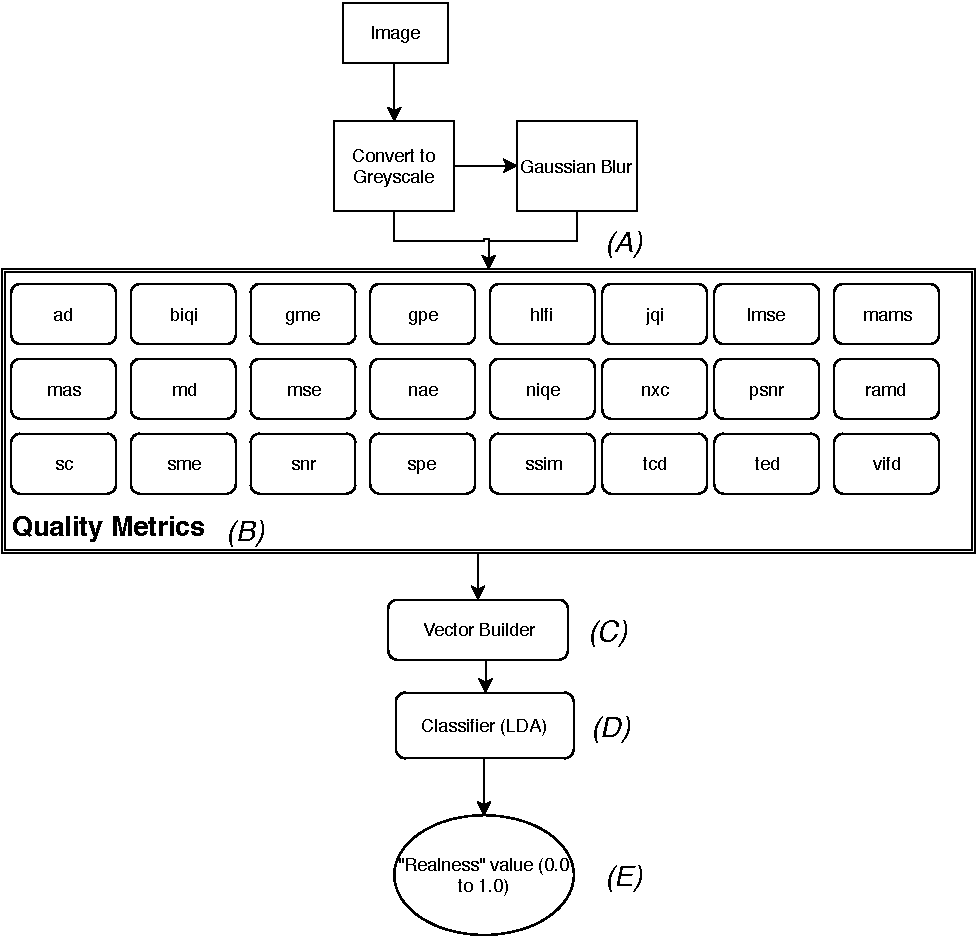
\includegraphics[width=.5\linewidth]{ImageQualityLivenessTest.pdf}
          \end{figure}
    
        \end{block}
       
        \begin{block}{Residual Networks for Facial Liveness}
          

          \begin{figure}
            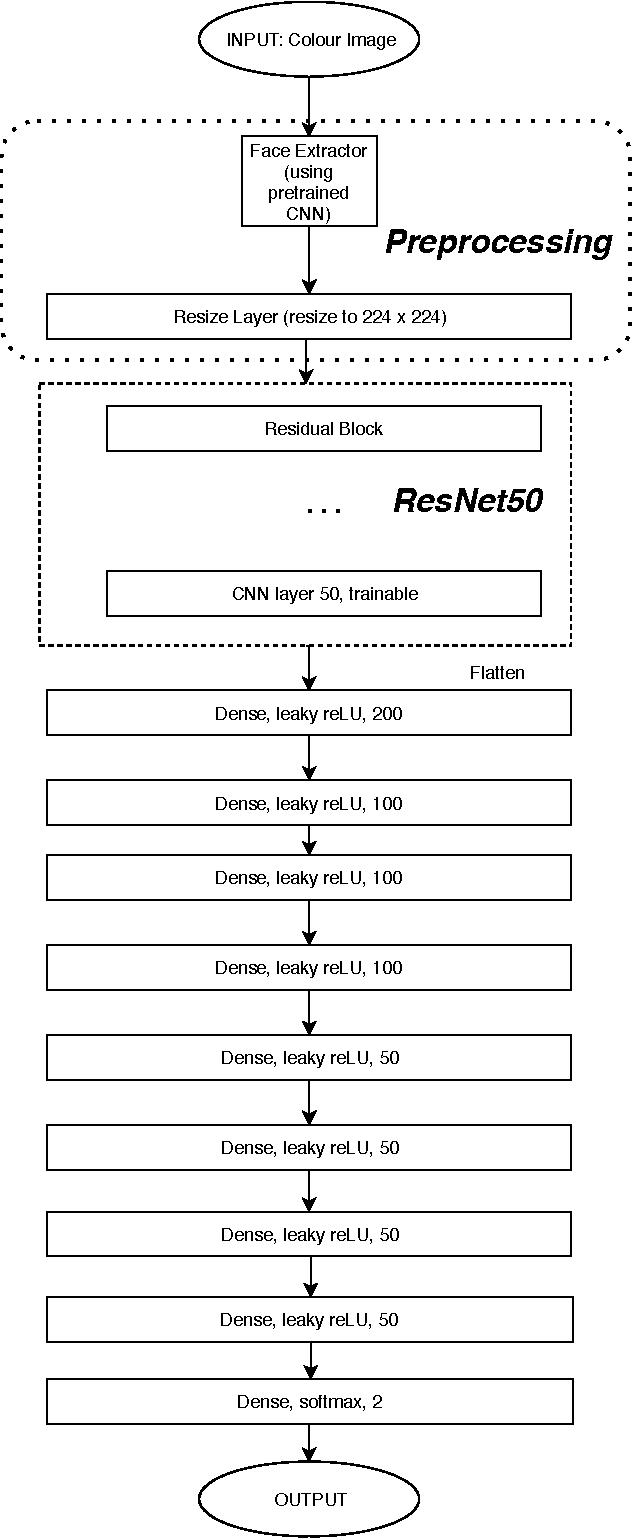
\includegraphics[height=450px]{2DCNNArchitecture.pdf}
          \end{figure}
    
        \end{block}

        \begin{block}{Facial reconstruction with classification from a 2D image}
          This was a proposed model that wasn't too effective based on the expected running times. Instead of the Replay-Attack or NUAA datasets,
          the Mask Attack Dataset was used since the goal of this classifier was to detect 3D based attacks.

          Given a 2D image, one can use pretrained neural network models to reconstruct the face in 3D. From here, this 3D representation could be
          classified.

          The reconstruction method used was VRN. This method produces a voxel representation which can then be classified. However, the time taken to
          reconstruct a single face with this model is 5 seconds, which is quite excessive for a production system for the web.

          The 3D classifier to use was VoxNet, since it performed adequately on the SUOD dataset. However, one major problem with dimensions occured: since the 3D reconstruction
          is of size 192x192, and this dimensionality is required, a large number of filters is needed for each convolution (192 filters to be precise). This led to a large
          memory complexity, meaning training was problematic. Decreasing the number of filters led to a model which wouldn't learn.

          While this model seemed like an interesting concept, and with more filters might perform adequately, in practice for production purposes it's not the most ideal solution.
          Therefore, this model isn't a suitable method to be included in such a system. However, future work could utilise 2D based CNN models (such as ResNet) to classify any 2D remnants of
          masks.
          
        \end{block}

        \begin{block}{Bringing several metrics together}
          Each individual liveness test produces some error in liveness classification. In order for a production system to be viable, this error needs to be reduced. Therefore, the solution is
          liveness test fusion: merging the results of different liveness tests together.

          Each liveness test has the option of producing a realness class (0 for fake, 1 for real), but using these integers as part of a sensor fusion system isn't ideal, since there's no measure
          of certainty. However, the probability of a classification can also be obtained, which ideally would yield a figure of 1 for real, or 0 for fake, or some number in between. However, the variance
          of each test isn't guaranteed, and specifically in the case of the WIQA method a fake image yields an output of 0.49, while a real image yields an output of 0.51. A fusion method should therefore be designed
          to take this into consideration.

          Initially, a perceptron was considered. For the two working metrics from above, the probabilities were plotted on a 2D chart. The probabilities themselves could be considered as linearly seperable, but
          when adding more and more nodes this might not be ideal (since it might be difficult for the classifier to learn a non-linearly seperable function space). As a result, an LDA was used.

          The LDA consolidation layer produced an accuracy of 0.75 which is improved over the individual metrics accuracy. However, it's hard to test the scalability here with only 2 livneess tests, so more work is needed to
          see how this scales.
        \end{block}

      \end{column}


      \begin{column}{.48\linewidth}

        \begin{block}{Evaluation}
          % TODO rewrite this
          \paragraph{Quality Test}
          The Quality Test performed well, and is suitable for a web based liveness service due to the high 87\% accuracy achieved.
          True positives and true negatives (that is, correct predictions for both real and fake) were high which means that the classifier
          is classifying correctly. However, the high false positive rate shows a slight cause for concern, since the model in 12.5\% of cases
          classified a fake image as real, which isn't ideal for our security focused solution. This could potentially be solved by adjusting output
          variable of the classifier (using a figure representing 'fakeness' rather than realness). This would hopefully lead to more false negatives,
          which are inconvenient but more secure for the system.

          In terms of computational performance, a 1.40 second time for classifying a single image is within the limits of the expected 2 seconds, and could be improved further
          with parallel based methods, and not relying on libsvm for the BIQI metric.
      \paragraph{2D CNN}
          The 2D CNN Test performed adequately. While the accuracy was lower than expected (at 71\%), the classifier itself still performed better than random.
          Furthermore, the model was very good at classifying true negatives, with a total percentage of 71.5\% being true negatives. While the model itself had
          a higher than expected false negative percentage, this is just inconvenient for the user rather than a security problem. The model showed it could classify true
          positives, but this figure was fairly low. This could be improved by improving the training process: ensuring each input image has a correctly identified face (as
          some images without a detectable face would have been left to classify the entire image, just resized to the input size). The less noise in the input data, the better the potential
          results in the future. Furthermore, using a larger ResNet model, such as ResNet-101 could lead to better results.

          In terms of performance, classifying an image is very quick, but the time taken to load the model is what took the most time (due to memory needing to be allocated and written to).
          In production, providing a model was preloaded and ready to accept input, the computation time of this metric would be very fast, and therefore be ideal for inclusion in a liveness web service.
      \paragraph{3D VoxNet Liveness Test}
          As seen from the results, this method of liveness test isn't feasible. With extra training, while the accuracy of the model could be improved, the
          real time memory requirements don't seem feasible. Based on the VoxNet paper, the accuracy achieved with a 32x32 VoxNet classifier on the SUOD dataset (a 3D dataset of objects)
          is 69\%. While this accuracy could be justified with reasonable computational and memory characteristics, this further proves that this method isn't feasible in the current state. In the future, a new approach of detecting 3D attacks is necessary.

        \end{block}
        
        \begin{block}{Conclusion}
          % TODO this needs to probably be reworded.
          This project showed that creating a facial liveness service for the web is a feasible idea, and performs fairly well for 2D attacks, with adequate accuracy and computational requirements.
          The image quality liveness test is accurate and fast, while the ResNet based method is a feasible idea and performs adequately, and could be improved further to improve the accuracy. For 3D attacks however, the
          proposed VoxNet based model performed badly and is not recommended for inclusion in a liveness test web service.

        \end{block}
      \end{column}
    \end{columns}

  % \vfill
  %   \begin{block}{\large This shows different font sizes you can use}
  %     \centering
  %     {\tiny tiny}\par
  %     {\scriptsize scriptsize}\par
  %     {\footnotesize footnotesize}\par
  %     {\normalsize normalsize}\par
  %     {\large large}\par
  %     {\Large Large}\par
  %     {\LARGE LARGE}\par
  %     {\veryHuge VeryHuge}\par
  %     {\VeryHuge VeryHuge}\par
  %     {\VERYHuge VERYHuge}\par
  %   \end{block}
  %   \vfill

  \end{frame}
\end{document}
